\documentclass[11pt]{article}
\usepackage[margin=2.3cm]{geometry}\usepackage{graphicx}\usepackage{booktabs}\usepackage{longtable}
\usepackage[T1]{fontenc}\usepackage[utf8]{inputenc}\usepackage{lmodern}\usepackage{microtype}
\usepackage[hidelinks]{hyperref}\usepackage{url}\usepackage{caption}\captionsetup{font=small}
\title{Off-street parking on rue de Terrebonne as built:\\ a reading of the 1954--55 fire-insurance plans}
\author{Terrebonne-open-sources (a resident of Côte-des-Neiges--Notre-Dame-de-Grâce)}
\date{October 25, 2026 \quad\small v2026-10-25-13-58-14}
\begin{document}\maketitle
\section*{Summary}
Of the \textbf{126} residential buildings with a rue de Terrebonne address between the west end of the protected lane (Belmore) and avenue Girouard on the sixteen sheets available, \textbf{75} were built with a garage, that is \textbf{60\,\%} (north side 57 of 90, 63\,\%; south side 18 of 36, 50\,\%). Counting only the readings made with high confidence gives 62\,\%. Weighted by the dwellings the City's assessment roll lists in the same buildings, 59\,\% of the 324 dwellings are in a building that was built with a garage.

The plans show garages as built, not driveways: a driveway without a garage leaves no mark, so the share of properties with a driveway or a garage as built is at least this figure. They show the stock of 1954--55, not of today; the City's roll dates 118 of the 121 matched buildings to 1955 or earlier (median 1932), so the frontage drawn is essentially the one standing today, but the use of each garage and driveway since then is not recorded here.

\section{Source}
The Underwriters' Survey Bureau, Limited, \emph{Insurance plan of the city of Montreal}, volume 7, sheets 739-2 to 739-5, 775, 784-1, 784-2, 785-1, 787-5 to 787-7, 789-12 to 789-16 and 798-3, dated November 1954 to December 1955 on the sheets (``Montreal, vol.~7, November 1954''; sheet 775 ``April 1955''; sheet 739-4 ``December 1955''). Each sheet carries the notice ``This plan is the property of the Underwriters' Survey Bureau, Limited, (unauthorized reproduction prohibited) \ldots'' and ``Copyright registered at Ottawa by the Underwriters' Survey Bureau, Limited, Toronto and Montreal''. The plans draw every building with its construction, storeys and civic number, and write \emph{Auto} or \emph{Autos} on every garage: in the basement (\emph{Auto Bt}, \emph{Autos Bast}), attached, or detached in the yard. The scans come from Biblioth\`eque et Archives nationales du Qu\'ebec (BAnQ num\'erique, collection \emph{Plans de villes et villages du Qu\'ebec}, notice 0000174390, 273 files, \url{https://collections.banq.qc.ca/ark:/52327/2244199}; rights statement \emph{Copyright Not Evaluated}); the full sheets are consulted there and not copied here. Sheet 787-8 (south side, Hampton to Melrose: the Royal and Draper blocks) is absent from BAnQ's file list (787-1 to 787-7 only) and from every other copy found; those two block faces are not counted (the north side opposite them has 15 garages on 17 buildings).

\section{Method}
\begin{enumerate}
\item \textbf{Reading.} Every building on the Terrebonne block faces, both sides, was read from the scans at two to four times magnification and recorded in \texttt{buildings\_1954.csv} (one row per building: sheet, side, block, cross streets, civic numbers, building type, the street it is addressed on, corner lot, garage yes/no, kind of garage, the presumed access, a confidence grade and notes). The unit is the building with a Terrebonne civic number: a semi-detached pair is two buildings, a duplex pair is one building of two to four flats, an apartment building counts once. Corner buildings addressed on the cross street (28, of which 13 with a garage) are listed with the cross street as their frontage and left out of the share; so are the two churches, the presbytery and the two frontages vacant in 1954--55.
\item \textbf{Georeferencing.} Each sheet was fitted to the City's géobase (CC-BY~4.0) by a similarity transform on the pixel positions of its Terrebonne intersections (\texttt{controls.csv}, \texttt{georef.py}); residuals are 0--4\,m (one of 7\,m). The fit was checked by drawing the City's assessment-roll parcels over each sheet.
\item \textbf{Positions and dwellings.} Each row was joined to the City's \emph{unités d'évaluation foncière} (CC-BY~4.0) by civic number and street, or, for corner buildings renumbered on the cross street since 1954, by position (\texttt{buildings.py}; 150 of 161 rows matched, the rest placed schematically along their block face). The roll gives the dwelling count and the year of construction of each matched building.
\item \textbf{Maps.} Both maps use a frame straightened along the street (distance along Terrebonne, offset across; north side above). The first draws the markers on the georeferenced sheets, the second on a base made only of the City's open data (\texttt{maps.py}).
\end{enumerate}

\section{Results}
\begin{table}[h]\centering\small
\begin{tabular}{lrrr}\toprule
 & Buildings addressed on Terrebonne & With a garage as built & Share\\\midrule
North side & 90 & 57 & 63\,\%\\
South side (sheet 787-8 missing) & 36 & 18 & 50\,\%\\
\textbf{Both sides} & \textbf{126} & \textbf{75} & \textbf{60\,\%}\\
High-confidence readings only & 97 & 60 & 62\,\%\\
Dwellings (City roll, 121 buildings) & 324 & 192 & 59\,\%\\\bottomrule
\end{tabular}\caption{Garages as built on the Terrebonne frontage, 1954--55 plans.}\end{table}

Of the 75 garages, 46 are basement garages, 14 are detached in the yard and 15 attached or in an annex. The door opens on Terrebonne for 64, on either street for 10 corner lots, and on a rear lane for 1. Building types on the frontage (from the plans): semi 38, single 15, duplex 67, row 2, apartment 4. Years of construction from the roll, by decade: 1910s 1, 1920s 29, 1930s 44, 1940s 15, 1950s 29, 1960s 1, 2000s 2.

\begin{longtable}{llp{5.2cm}rrr}
\caption{By block face (residential buildings addressed on Terrebonne).}\\\toprule
Side & Sheet & Block face & Buildings & Garage & Share\\\midrule\endfirsthead
\toprule Side & Sheet & Block face & Buildings & Garage & Share\\\midrule\endhead
N & 789-12 & Belmore-Coronation & 3 & 1 & 33\,\% \\
N & 789-13 & Coronation-Mayfair & 6 & 0 & 0\,\% \\
N & 789-13 & Mariette-Rosedale & 2 & 2 & 100\,\% \\
N & 789-14 & Rosedale-King Edward & 5 & 4 & 80\,\% \\
N & 789-14 & King Edward-Montclair & 2 & 1 & 50\,\% \\
N & 789-14 & Montclair-Walkley & 3 & 1 & 33\,\% \\
N & 789-15 & Walkley-Prince of Wales & 3 & 3 & 100\,\% \\
N & 789-15 & Cumberland-Cavendish & 2 & 2 & 100\,\% \\
N & 789-16 & Cavendish-Bessborough & 4 & 0 & 0\,\% \\
N & 789-16 & Bessborough-Benny & 2 & 0 & 0\,\% \\
N & 798-3 & Benny-Madison & 2 & 2 & 100\,\% \\
N & 798-3 & Madison-Kensington & 4 & 0 & 0\,\% \\
N & 798-3 & Kensington-Grand & 1 & 1 & 100\,\% \\
N & 787-5 & Grand-Beaconsfield & 4 & 1 & 25\,\% \\
N & 787-5 & Beaconsfield-Hingston & 6 & 5 & 83\,\% \\
N & 787-5 & Hingston-Hampton & 9 & 9 & 100\,\% \\
N & 787-6 & Hampton-Royal & 7 & 5 & 71\,\% \\
N & 787-6 & Royal-Draper & 6 & 6 & 100\,\% \\
N & 787-6 & Draper-Melrose & 4 & 4 & 100\,\% \\
N & 739-2 & Melrose-Wilson & 1 & 1 & 100\,\% \\
N & 739-2 & Wilson-Harvard & 3 & 2 & 67\,\% \\
N & 739-2 & Harvard-Oxford & 3 & 3 & 100\,\% \\
N & 739-5 & Oxford-Marcil & 4 & 0 & 0\,\% \\
N & 739-5 & Marcil-Old Orchard & 2 & 2 & 100\,\% \\
N & 739-5 & Old Orchard-Hampstead apts & 1 & 1 & 100\,\% \\
N & 739-5 & Old Orchard-Girouard & 1 & 1 & 100\,\% \\
S & 784-1 & Coronation-Mayfair & 4 & 2 & 50\,\% \\
S & 784-2 & Mayfair-Mariette & 3 & 2 & 67\,\% \\
S & 784-2 & Rosedale-King Edward & 2 & 0 & 0\,\% \\
S & 785-1 & King Edward-Montclair & 2 & 2 & 100\,\% \\
S & 785-1 & Montclair-Walkley & 1 & 0 & 0\,\% \\
S & 785-1 & Walkley-Prince of Wales & 2 & 2 & 100\,\% \\
S & 785-1 & Prince of Wales-Cumberland & 1 & 1 & 100\,\% \\
S & 785-1 & Cumberland-Cavendish & 3 & 0 & 0\,\% \\
S & 775 & Cavendish-Madison & 1 & 0 & 0\,\% \\
S & 775 & Madison-Kensington & 3 & 2 & 67\,\% \\
S & 787-7 & Grand-Beaconsfield & 3 & 1 & 33\,\% \\
S & 787-7 & Beaconsfield-Hingston & 3 & 3 & 100\,\% \\
S & 787-7 & Hingston-Hampton & 3 & 2 & 67\,\% \\
S & 739-4 & west cross street-Oxford & 3 & 1 & 33\,\% \\
S & 739-5 & Oxford-Marcil & 1 & 0 & 0\,\% \\
S & 739-5 & Old Orchard-Girouard & 1 & 0 & 0\,\% \\
\\\bottomrule\end{longtable}

\begin{figure}[p]\centering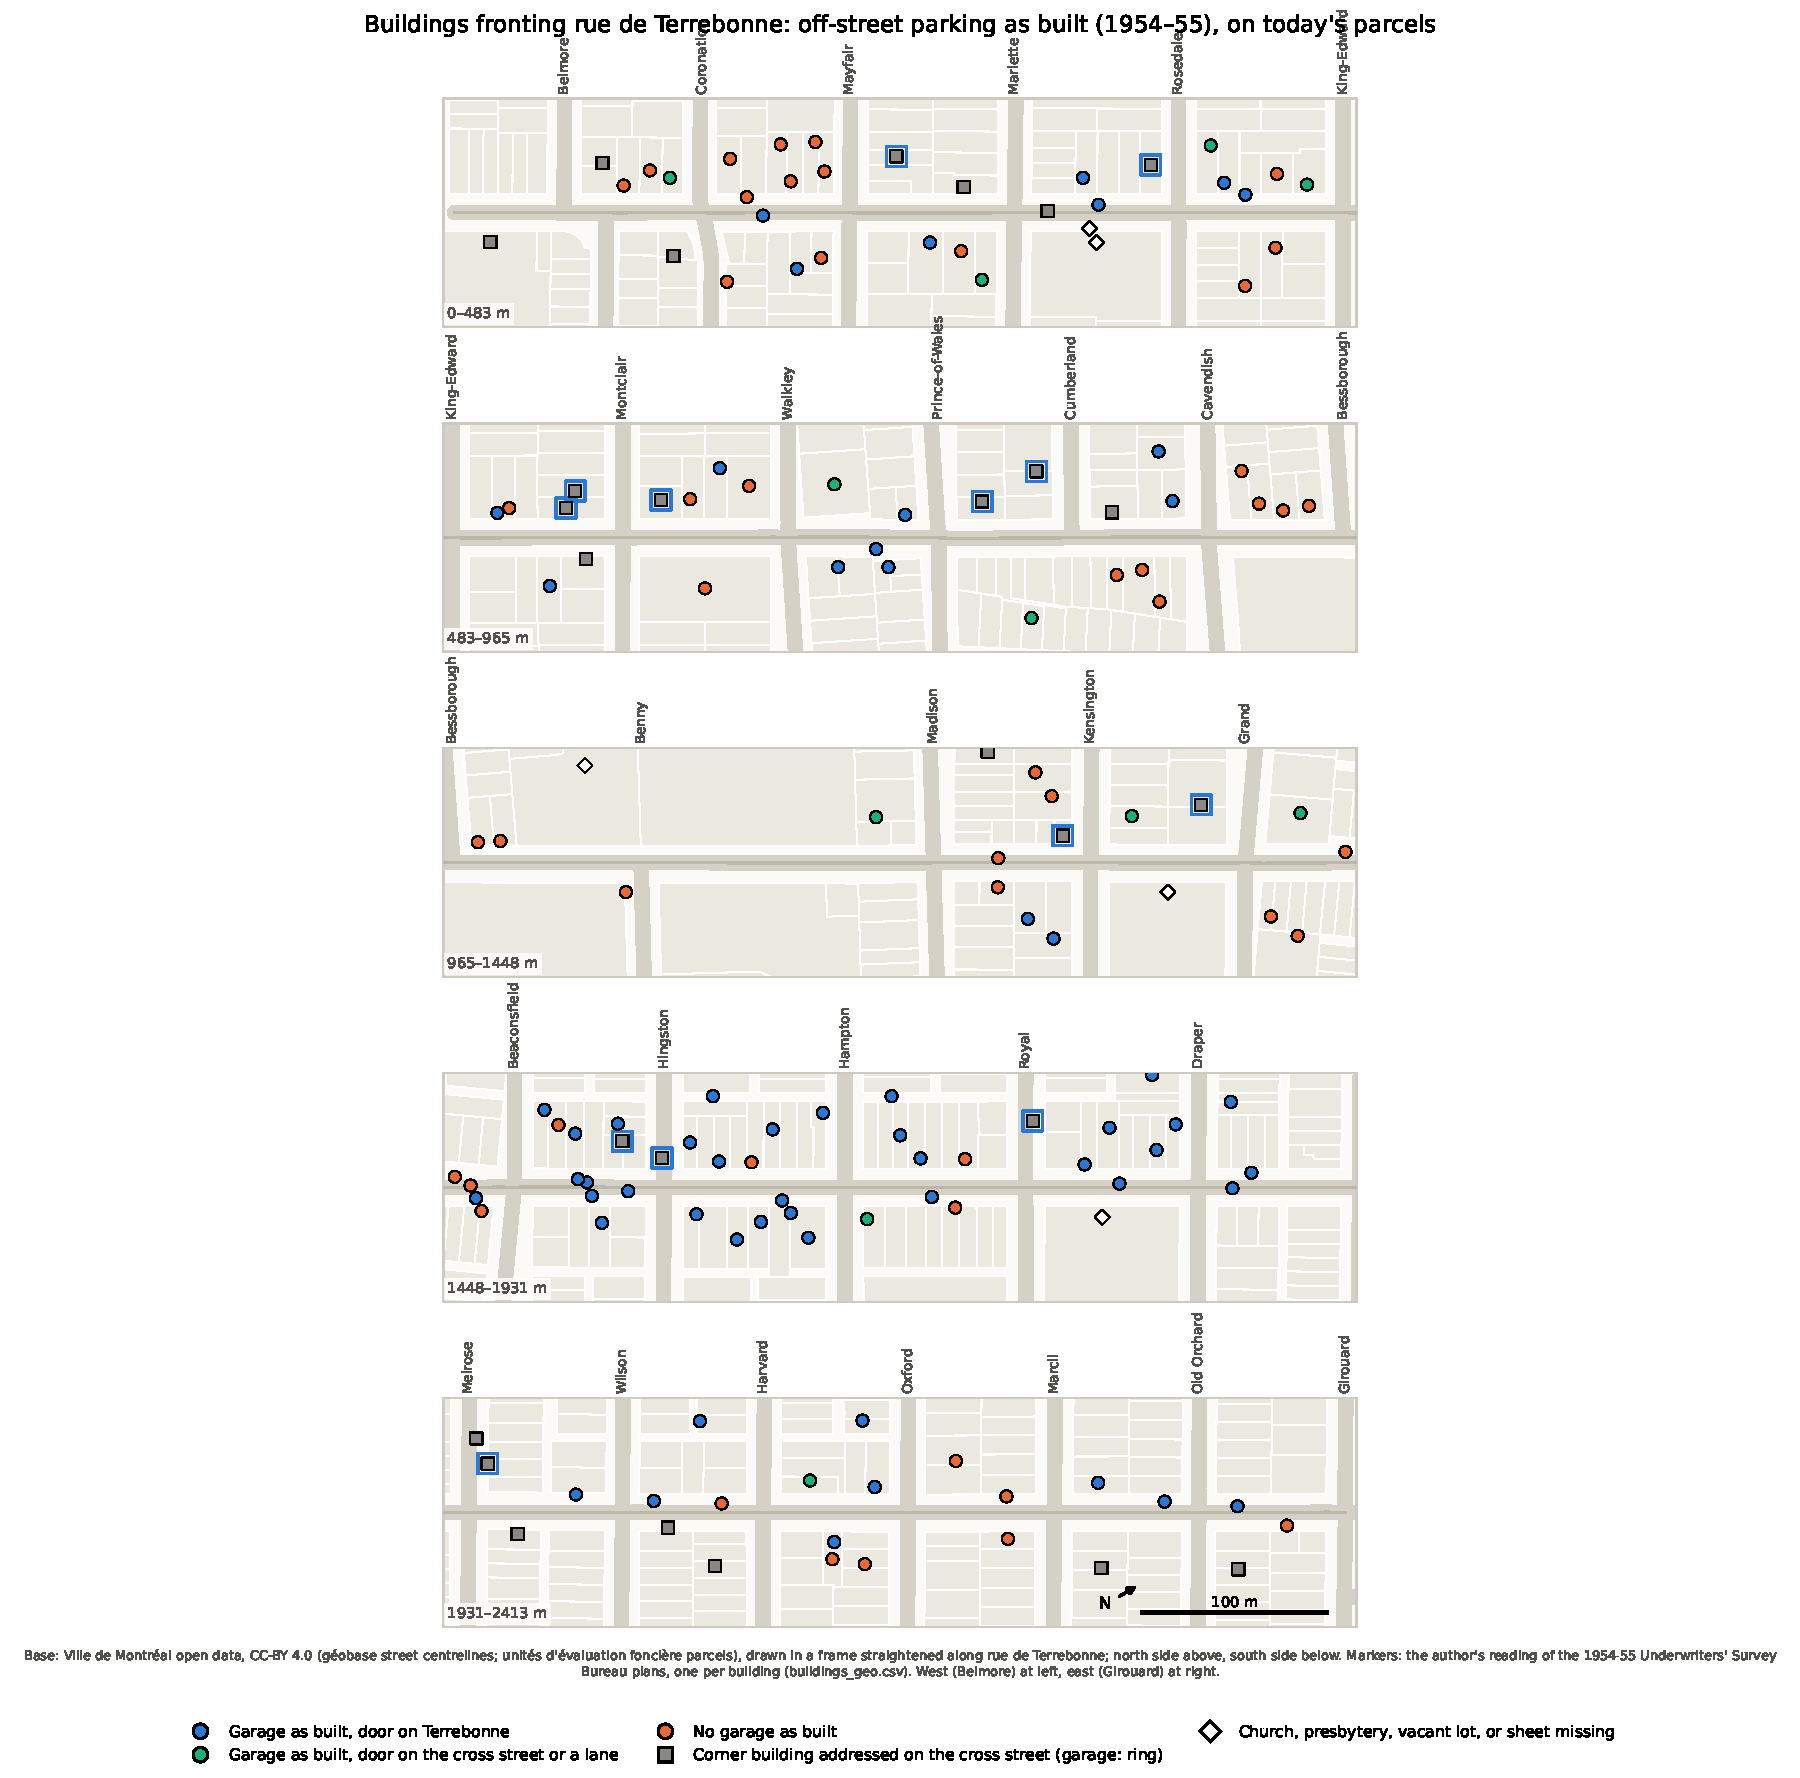
\includegraphics[width=\textwidth]{figures/terrebonne_garages_1954_map_city_en.pdf}
\caption{On a base drawn from the City's open data (géobase, assessment-roll parcels; CC-BY 4.0).}\end{figure}
\begin{figure}[p]\centering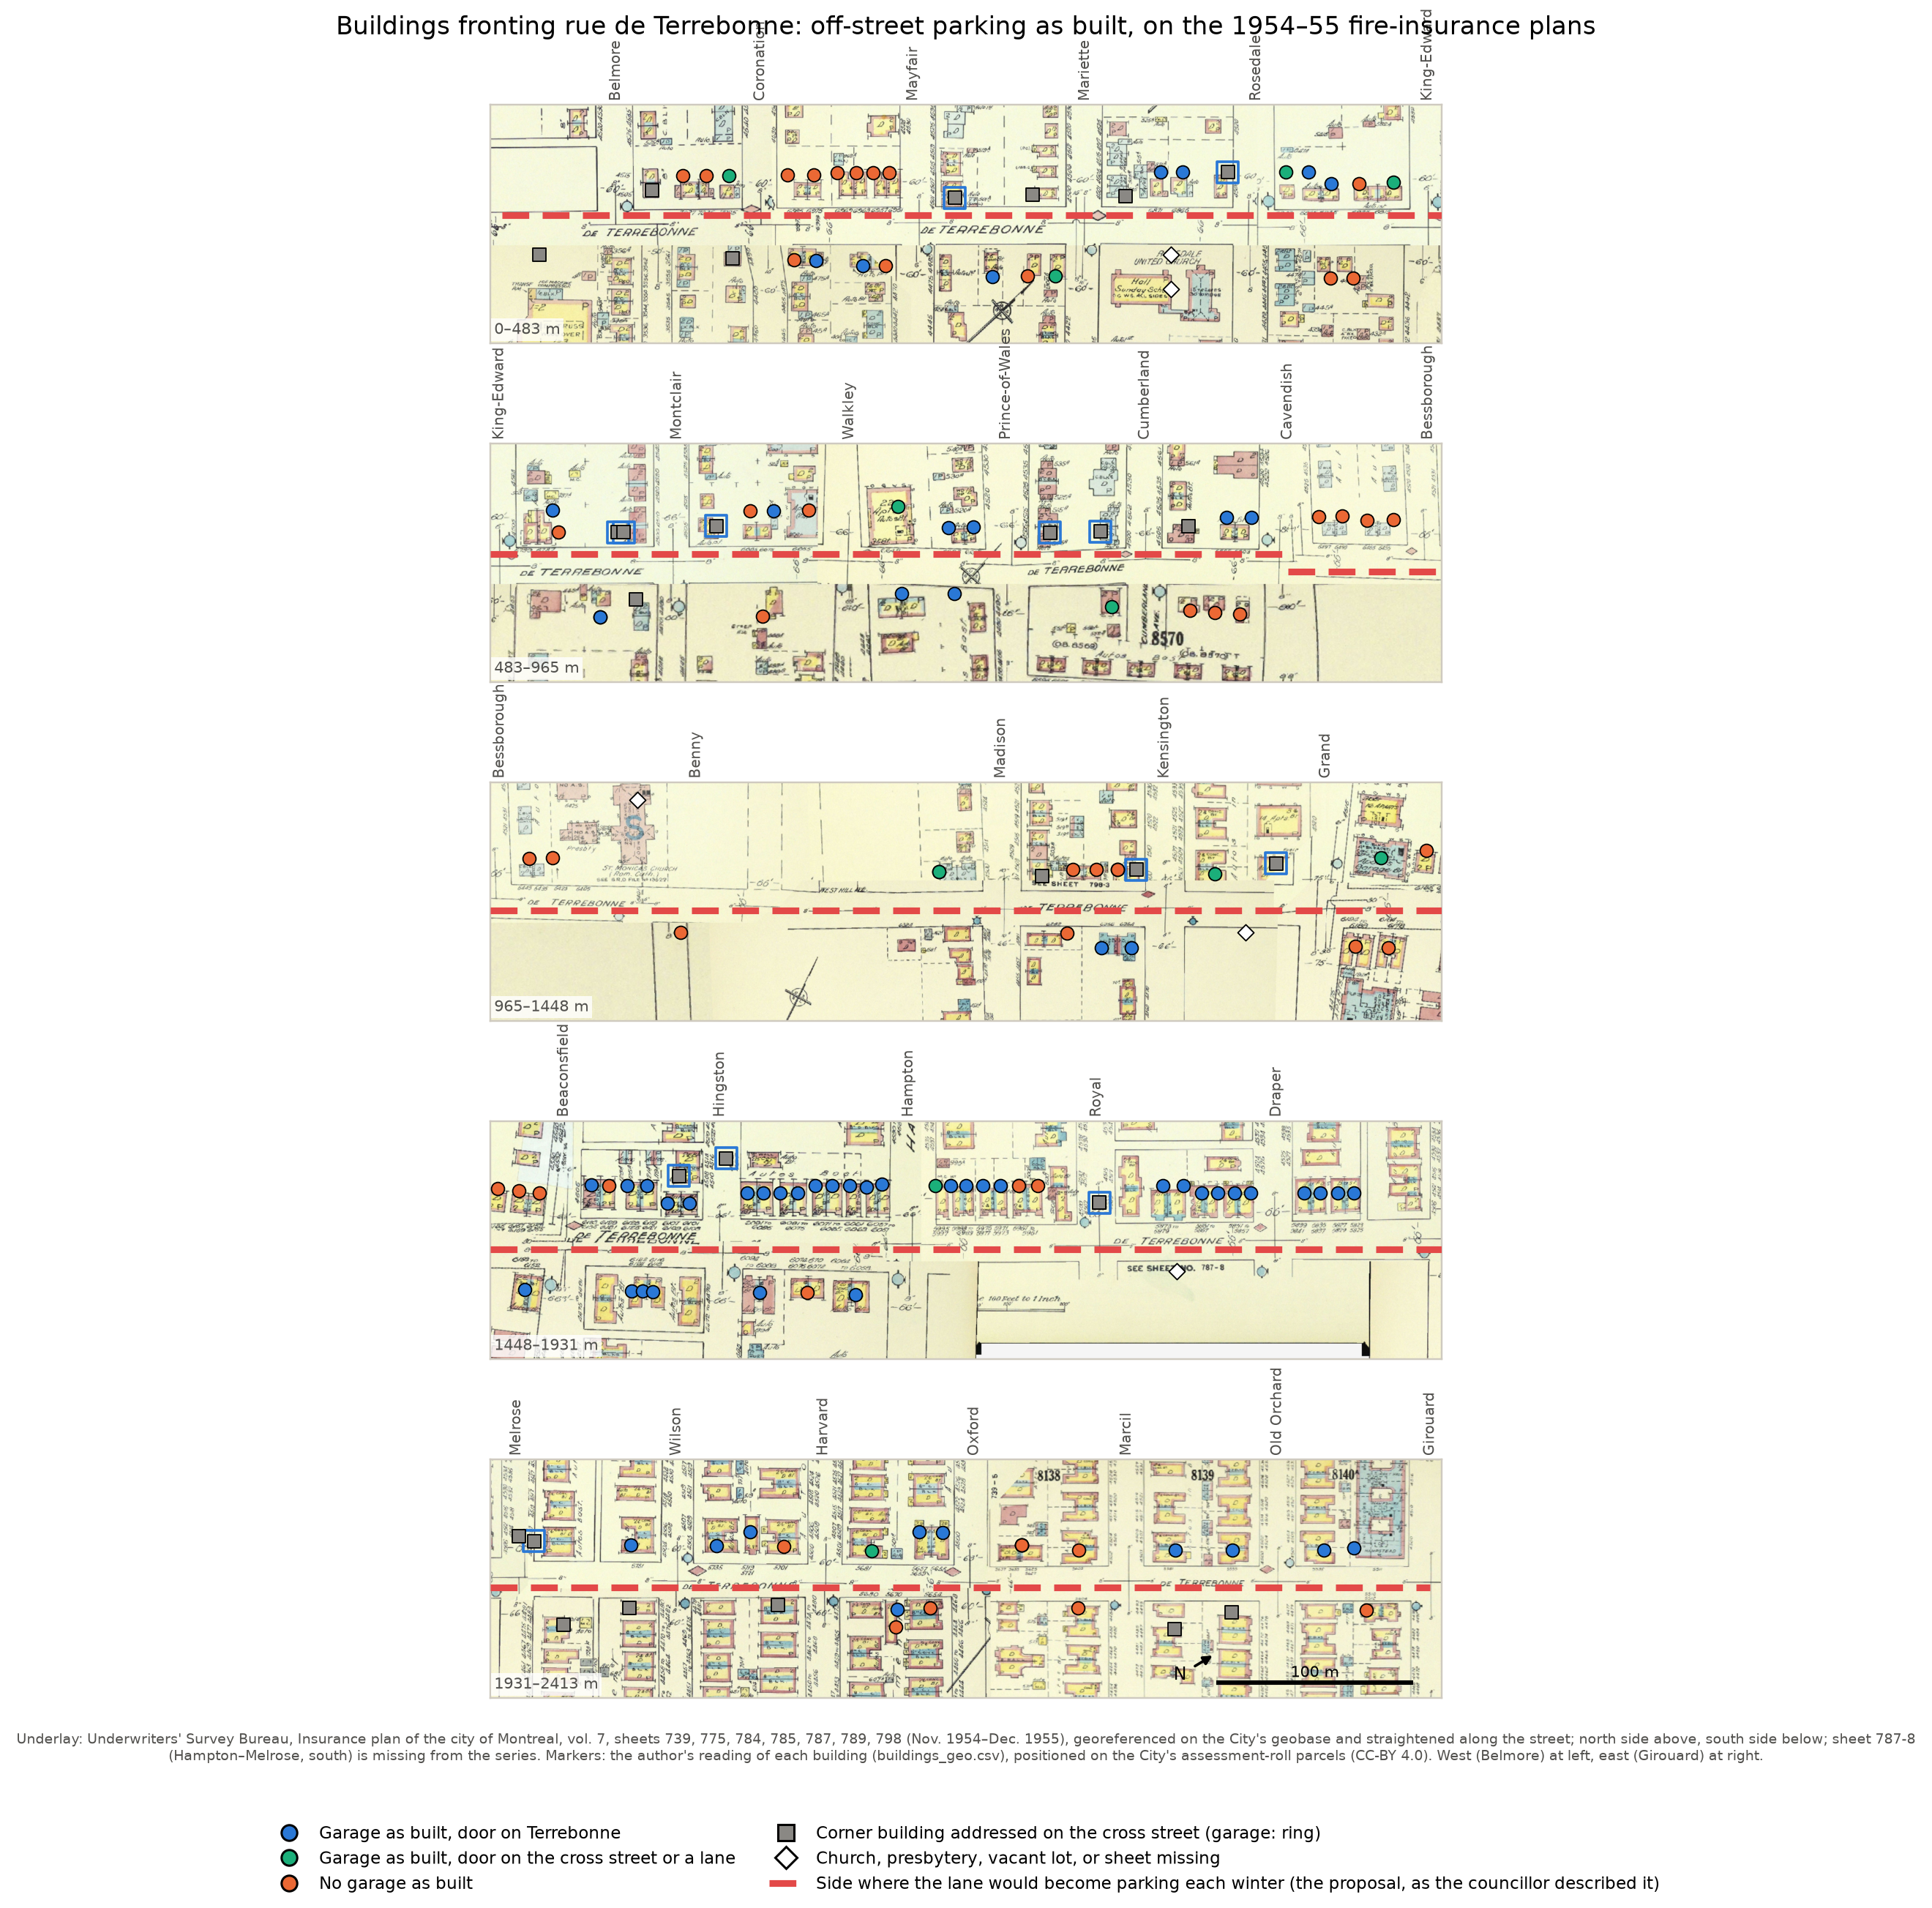
\includegraphics[width=\textwidth]{figures/terrebonne_garages_1954_map_underwriters_en.png}
\caption{On the 1954--55 sheets, georeferenced and straightened along the street.}\end{figure}

\section{The frontages today}
A check of each building's frontage on the Gouvernement du Qu\'ebec's continuous aerial imagery (service \emph{Imagerie\_GQ}, fetched October 25, 2026; leaf-off spring imagery, about 8~cm per pixel; the City's parcels overlaid) recorded, for 123 of the 126 buildings, whether a driveway, paved apron or parking pad is visible on the lot today, whether a vehicle was parked on it at the moment of the photograph, and from which street it is reached (\texttt{buildings\_geo.csv}, columns \texttt{driveway\_today}, \texttt{vehicle\_or\_pad\_on\_lot}, \texttt{access\_today}). What a garage holds inside cannot be seen from above, so the check measures the visible access, not the use.

\begin{table}[h]\centering\small
\begin{tabular}{lrr}\toprule
 & Buildings & Share\\\midrule
Checked & 123 & \\
Driveway, apron or parking pad visible today & 79 & 64\,\%\\
Garage as built (1954--55) \emph{or} driveway today & 89 & 72\,\%\\
\quad north side & 70 of 89 & 79\,\%\\
\quad south side & 19 of 34 & 56\,\%\\
\quad by dwellings (City roll) & 221 of 303 & 73\,\%\\
Garage of 1954--55 with its apron still visible & 64 & \\
Garage of 1954--55 with no apron visible today & 10 & \\
No garage in 1954--55, a driveway or pad today & 15 & \\
A vehicle parked on the lot when photographed & 34 & \\\bottomrule
\end{tabular}\caption{The frontages today (aerial imagery read October 25, 2026).}\end{table}

\begin{figure}[p]\centering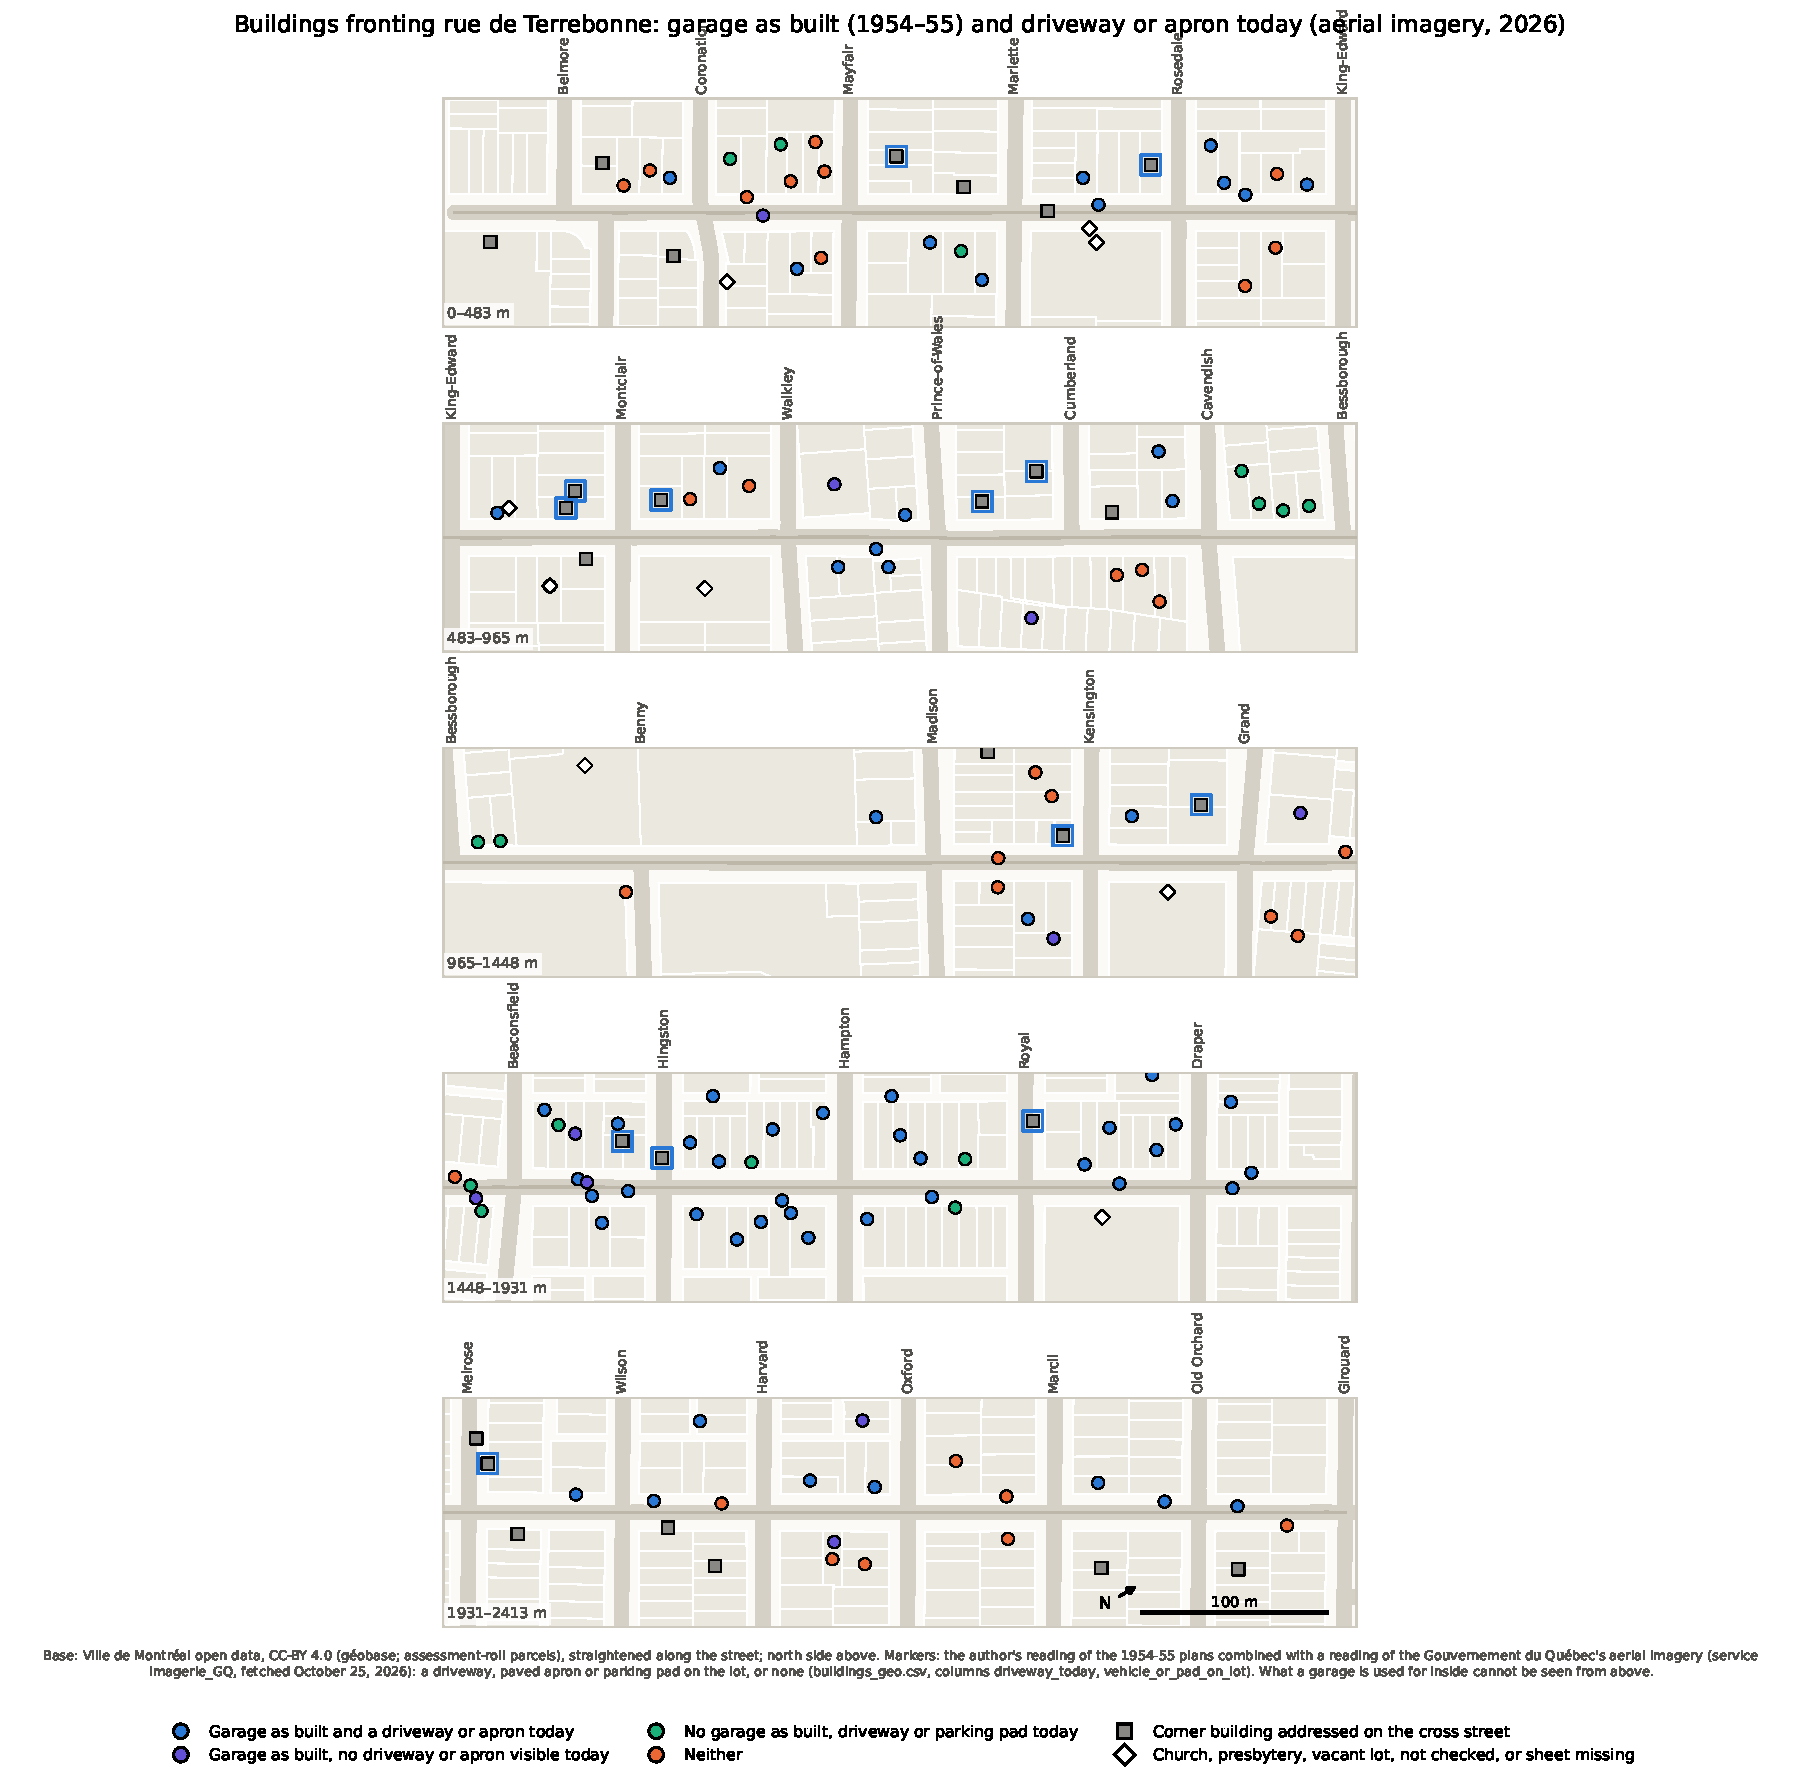
\includegraphics[width=\textwidth]{figures/terrebonne_garages_1954_map_today_en.pdf}
\caption{Garage as built and driveway today, building by building.}\end{figure}

\section{Caveats}
\begin{itemize}
\item \textbf{Garages, not driveways.} The plans mark structures. A driveway or parking pad without a garage leaves no mark, so the as-built share with a driveway or garage is a lower bound.
\item \textbf{As built, not as used.} The 1954--55 share counts structures; the present-day check sees aprons, driveways and parked vehicles from above but not what a garage holds inside (a workshop, storage, living space), so neither figure is the share of households that park off-street today. A garage built in 1930 or 1950 may also be too small for a large vehicle of today. Ten garages of 1954--55 show no apron today and one reading is unclear.
\item \textbf{Buildings, not households.} The share by building and the share by dwelling happen to agree (60\,\% and 59\,\%), but a duplex pair has two to four flats and one or two garages, and three of the four apartment buildings have a basement garage of unrecorded capacity.
\item \textbf{One sheet missing} (787-8) and 29 readings graded medium (noted row by row).
\item \textbf{Corner lots.} Which street a corner building is addressed on changed in places between 1954 and the present roll; the table keeps the 1954 numbering and the join records the present unit.
\end{itemize}
\end{document}
